% Bachelorproef - Verdediging
% Geautomatiseerde security assessment van MCP-servers in Fintech

\documentclass[aspectratio=169]{beamer}

% Layout
\usetheme{hogent}
\usecolortheme{hgwhite}      % of hgblack voor donkere achtergrond

% Packages
\usepackage{babel}
\babelprovide[main, import]{dutch}
\usepackage{booktabs}
\usepackage{multirow,multicol}
\usetikzlibrary{calc}
\graphicspath{{graphics/}}

% Hulpmacro: volledige afbeelding of nette placeholder als ze nog ontbreekt.
\newcommand{\fullimage}[1]{%
  \IfFileExists{graphics/#1}%
    {\includegraphics[width=\paperwidth,height=\paperheight,keepaspectratio]{#1}}%
    {\centering\vfill{\large\textcolor{hggrey}{[\,afbeelding: #1\,]}}\vfill}%
}

% Poster-navigator uitgeschakeld: stond rechtsonder in de weg van de tekst.
% De \posternav-aanroepen op de slides blijven staan maar doen niets meer.
\newcommand{\posternav}[4]{}

% Metadata
\title{Geautomatiseerde security assessment van MCP-servers}
\subtitle{Verdediging bachelorproef Toegepaste Informatica}
\author{Arthur Van Oudenhove}
\date{\today}

\begin{document}

% Titeldia
{
  \setbeamertemplate{background}[imgletter]{blurred-background-cellphone-coffee-842554.jpg}{A}
  \begin{frame}
    \maketitle
  \end{frame}
}

\begin{frame}
  \frametitle{Overzicht.}
  \tableofcontents
\end{frame}

\section{Introductie}

% Slide 2: de poster als totaalbeeld
\begin{frame}[plain]
  \fullimage{poster-full.png}
\end{frame}
% Spreektekst (~1:30): "Dit is het hele plaatje. Probleem, aanpak, resultaten,
% conclusie. Ik loop het nu hoofdstuk per hoofdstuk met u door."

% Slide 3: probleem
\begin{frame}
  \frametitle{AI-agents in Fintech, via MCP.}
  \begin{itemize}
    \item AI-agents verwerken betalingen en bedrijfskritische taken.
    \item Communicatie met interne systemen loopt via het \textbf{Model Context Protocol}.
    \item Standaardisatie opent nieuwe aanvalsvlakken:
      \emph{prompt injection} $\cdot$ \emph{tool poisoning} $\cdot$ \emph{privilege escalation}.
  \end{itemize}
  \vfill
  \centering\textbf{56\% van de bedrijven met AI-agents rapporteert MCP-beveiligingsincidenten.}
  \posternav{0.03}{0.58}{0.49}{0.72}   % Introductie (boven): probleem
  \note{Fintech-groei $\cdot$ MCP = standaard $\cdot$ keerzijde = aanvalsvlak}
\end{frame}

% Slide 4: onderzoeksvraag en scope
\begin{frame}
  \frametitle{Onderzoeksvraag.}
  \textbf{\textcolor{hgdarkgreen}{Hoofdvraag:}} hoe kan een framework MCP-servers
  automatisch testen op een set kritieke kwetsbaarheden, en hoe verhoudt
  dekkingsgraad en tijd zich tot een handmatige beoordeling?
  \vfill
  \textbf{Scope:} \'e\'en gecontroleerde evaluatiecase, de opzettelijk
  kwetsbare \emph{Goat}-server met een vaste ground truth.
  \posternav{0.03}{0.34}{0.49}{0.46}   % Onderzoeksvraag en aanpak (kop)
  \note{vraag groot $\cdot$ scope eerlijk = \'e\'en case $\cdot$ niet "MCP-breed"}
\end{frame}

\section{Aanpak}

% Slide 5: de leemte
\begin{frame}
  \frametitle{Waarom generieke tools tekortschieten.}
  \begin{columns}[T]
    \column{.5\textwidth}
      \textbf{Burp Suite}
      \begin{itemize}
        \item ziet HTTP/JSON-RPC,
        \item maar kent de \textbf{semantiek} van MCP-schema's niet.
      \end{itemize}
    \column{.5\textwidth}
      \textbf{Semgrep}
      \begin{itemize}
        \item detecteert code-patronen,
        \item maar niet de \textbf{runtime}-interactie agent$\leftrightarrow$server.
      \end{itemize}
  \end{columns}
  \vfill
  \centering\textbf{Geen contextuele kennis van MCP-specifieke kwetsbaarheden.}
  \posternav{0.03}{0.45}{0.49}{0.58}   % Introductie (onder): leemte
\end{frame}

% Slide 6: architectuur
\begin{frame}
  \frametitle{Architectuur.}
  \vfill
  \centering
  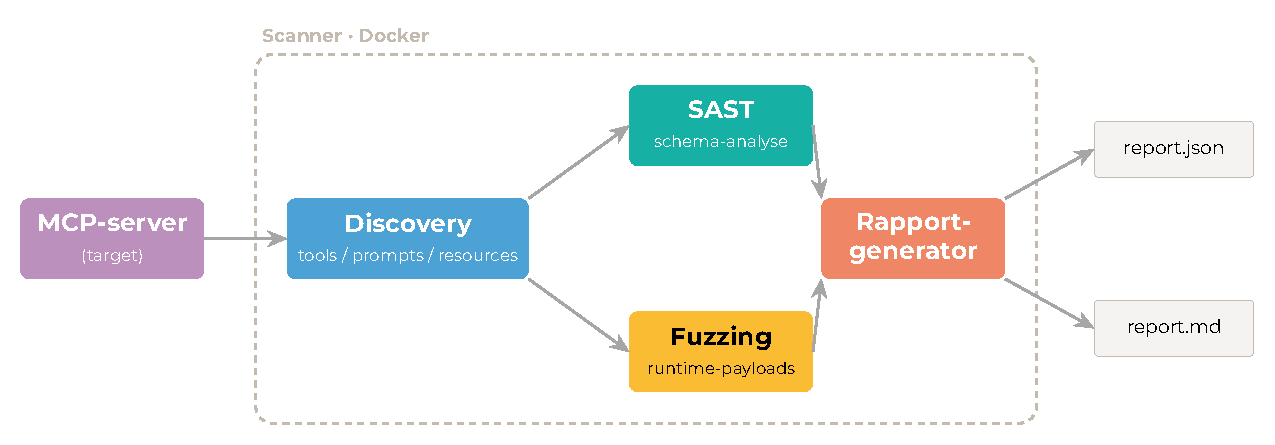
\includegraphics[width=0.95\linewidth]{architectuur.pdf}
  \vfill
  \note{discovery $\cdot$ statisch + dynamisch $\cdot$ uniform Finding $\cdot$ Docker}
\end{frame}

% Slide 7: detectie-aanpak
\begin{frame}
  \frametitle{Statisch \'en dynamisch.}
  \begin{columns}[T]
    \column{.5\textwidth}
      \textbf{\textcolor{hgdarkgreen}{SAST (schema)}}
      \begin{itemize}
        \item prompt injection in beschrijving
        \item ontbrekende autorisatiecontext
        \item ongebonden parameters
      \end{itemize}
    \column{.5\textwidth}
      \textbf{\textcolor{hgblue}{Fuzzing (runtime)}}
      \begin{itemize}
        \item information disclosure
        \item injection-reflectie
        \item autorisatiebypass / tool poisoning
      \end{itemize}
  \end{columns}
  \vfill
  \centering Runtime-gedrag is onzichtbaar in broncode, daarom allebei.
  \posternav{0.03}{0.19}{0.49}{0.34}   % Aanpak: detectieregels
\end{frame}

\section{Demo \& resultaten}

% Slide 8: demo
\begin{frame}[plain]
  \centering
  \fullimage{demo-still.png}
  \vfill
  {\Large \textcolor{hgorange}{$\blacktriangleright$\ demo (screencast)}}
  \note{NIET embedden: speel los .mp4 af $\cdot$ narreren: scan Goat -> 5 lekken -> rapport}
\end{frame}

% Slide 9: resultaten Goat
\begin{frame}
  \frametitle{Resultaten op Goat.}
  \centering
  \begin{tabular}{@{}lcc@{}}
    \toprule
    \textbf{Meetdimensie} & \textbf{Framework} & \textbf{Handmatig} \\ \midrule
    Recall                & \textcolor{hgdarkgreen}{100\% (5/5)} & 80\% (4/5) \\
    Precisie              & \textcolor{hgdarkgreen}{$\geq$92,3\% (12/13)} & 100\% (4/4) \\
    Benodigde tijd        & \textcolor{hgdarkgreen}{$<$30 sec} & 47 min \\
    Reproduceerbaarheid   & gegarandeerd       & afhankelijk van reviewer \\ \bottomrule
  \end{tabular}
  \vfill
  \centering Het tijdsverschil (factor $\sim$90) is reviewer-onafhankelijk.
  \posternav{0.03}{0.02}{0.49}{0.19}   % Resultaten (grafiek, linksonder)
\end{frame}

\section{Validatie op een echte server}

% Slide 10: Zowe (na indiening)
\begin{frame}
  \frametitle{Na indiening: een \'echte server.}
  \begin{flushright}\small\textcolor{hgorange}{\textbf{[ werk na indiening ]}}\end{flushright}
  \textbf{Vraag:} werkt het buiten de benchmark?
  \medskip
  \begin{itemize}
    \item Target: officiële \textbf{Zowe MCP-server} (mainframe, mock-modus).
    \item Streamable HTTP, 62 tools ontdekt.
    \item Resultaat: $\sim$249 bevindingen.
  \end{itemize}
  \vfill
  \centering\textbf{Precisie stort in: van 92,3\% op Goat naar bijna nul hier. Waarom?}
  \note{eerlijk labelen: na indiening $\cdot$ echte, niet-kwetsbare server}
\end{frame}

% Slide 11: tier-tabel, de kernslide
\begin{frame}
  \frametitle{De findings volgen de policy, niet de kwetsbaarheden.}
  \centering
  \begin{tabular}{@{}lccc@{}}
    \toprule
    \textbf{Capability-tier} & \textbf{Tools} & \textbf{Totaal findings} & \textbf{waarvan HIGH ``autorisatie''} \\ \midrule
    read(-strict) & 31 & 106 & 36 \\
    update        & 49 & 196 & 62 \\
    delete        & 55 & 227 & 74 \\
    \textbf{full} & \textbf{62} & \textbf{249} & \textbf{83} \\ \bottomrule
  \end{tabular}
  \vfill
  \centering\textbf{De bevindingen schalen met de operator-policy, niet met de
  beveiligingsstaat.}\\ Het scherpste bewijs dat het false positives zijn.
  \note{kern: heuristiek zoekt auth in schema; Zowe autoriseert op tier/transport}
\end{frame}

\section{Reflectie \& conclusie}

% Slide 12: kritische reflectie
\begin{frame}
  \frametitle{Kritische reflectie.}
  \begin{itemize}
    \item \textbf{Circulaire benchmark:} Goat is ontworpen voor mijn regels,
          dus 100\% recall is best-case.
    \item \textbf{n=1 reviewer:} handmatige vergelijking is illustratief, niet
          statistisch valide.
    \item \textbf{Externe validiteit:} hoge recall, lage precisie buiten de
          benchmark (zie Zowe).
  \end{itemize}
  \posternav{0.52}{0.42}{0.98}{0.72}   % Conclusies (boven)
\end{frame}

% Slide 13: aanbevelingen
\begin{frame}
  \frametitle{Aanbevelingen.}
  \begin{itemize}
    \item Screeningslaag in CI/CD, \textbf{geen} vervanging van een audit.
    \item Dwing autorisatie af op elke gevoelige tool.
    \item Behandel tool-outputs als onvertrouwde invoer.
    \item Elke run vraagt een menselijke triagefase.
  \end{itemize}
  \posternav{0.52}{0.20}{0.98}{0.42}   % Conclusies/aanbevelingen (onder)
\end{frame}

% Slide 14: conclusie
\begin{frame}
  \frametitle{Conclusie.}
  \centering\large
  Geautomatiseerde MCP-assessment is \textbf{haalbaar} en \textbf{snel},
  met hoge recall op de doelklasse.\\[1ex]
  De \textbf{grens}, de precisie buiten de benchmark, is even eerlijk in
  kaart gebracht.
  \vfill
  \normalsize Toekomstig werk: evaluatie op MCPTox (45 re\"ele servers).
  \posternav{0.52}{0.20}{0.98}{0.72}   % Rechterkolom: conclusie
\end{frame}

% Back-up (starred: geen tussendia, niet in inhoudsopgave)
\section*{Back-up}

\begin{frame}
  \frametitle{Back-up: OWASP MCP Top 10 mapping.}
  \begin{itemize}
    \item Tool poisoning $\rightarrow$ \textbf{MCP03}
    \item Ontbrekende autorisatie $\rightarrow$ \textbf{MCP07}
    \item Privilege escalation $\rightarrow$ \textbf{MCP02}
    \item Prompt injection $\rightarrow$ \textbf{Intent Flow Subversion}
  \end{itemize}
\end{frame}

\begin{frame}
  \frametitle{Back-up: Zowe-adapter \& transport.}
  \begin{itemize}
    \item Streamable HTTP: \texttt{initialize} $\rightarrow$ \texttt{mcp-session-id} $\rightarrow$ \texttt{tools/list}.
    \item Adapter uitgebreid met Accept-header + SSE-parsing (na indiening).
  \end{itemize}
\end{frame}

\begin{frame}
  \frametitle{Back-up: scope \& beperkingen.}
  \begin{itemize}
    \item Geen geauthenticeerde scanning.
    \item Enkel HTTP/SSE-transport (geen stdio).
    \item Point-in-time, geen continue monitoring.
  \end{itemize}
\end{frame}

\end{document}
